\begin{figure}[h]
	\centering
	\makebox[0.11\textwidth]{\tiny 图像}
	\enspace
	\makebox[0.11\textwidth]{\tiny 真值}
	\enspace
	\makebox[0.11\textwidth]{\tiny CNN+5LSTM\textbf{1}}
	\enspace\thinspace
	\makebox[0.11\textwidth]{\tiny CNN+5LSTM\textbf{2}}
	\enspace\thinspace
	\makebox[0.11\textwidth]{\tiny CNN+5LSTM\textbf{3}}
	\enspace\thinspace
	\makebox[0.11\textwidth]{\tiny CNN+5LSTM\textbf{4}}
	\enspace\thinspace
	\makebox[0.11\textwidth]{\tiny CNN+5LSTM\textbf{5}}\\
	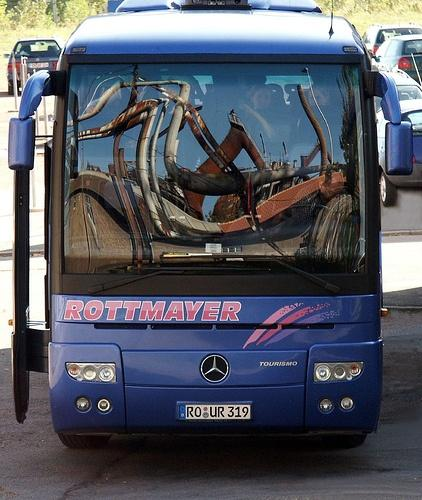
\includegraphics[width=0.11\textwidth]{demo_images/improvement/2007_000663.jpg}
	\enspace\enspace %\hfill
	
\includegraphics[width=0.11\textwidth]{demo_images/improvement/2007_000663.png}
	\enspace\enspace
	
\includegraphics[width=0.11\textwidth]{demo_images/improvement/2007_000663_1.png}
	\enspace\enspace
	
\includegraphics[width=0.11\textwidth]{demo_images/improvement/2007_000663_2.png}
	\enspace\enspace
	
\includegraphics[width=0.11\textwidth]{demo_images/improvement/2007_000663_3.png}
	\enspace\enspace
	
\includegraphics[width=0.11\textwidth]{demo_images/improvement/2007_000663_4.png}
	\enspace\enspace
	
\includegraphics[width=0.11\textwidth]{demo_images/improvement/2007_000663_5.png}
	\enspace\enspace
	\caption[同一网络网格型长短记忆网络时序的增加对输出改善作用的可视化]{网格型长短记忆网络层数增加对输出改善作用的可视化}
	\label{fig:improvement}
\end{figure}